\documentclass[tikz,border=10pt]{standalone}
\begin{document}
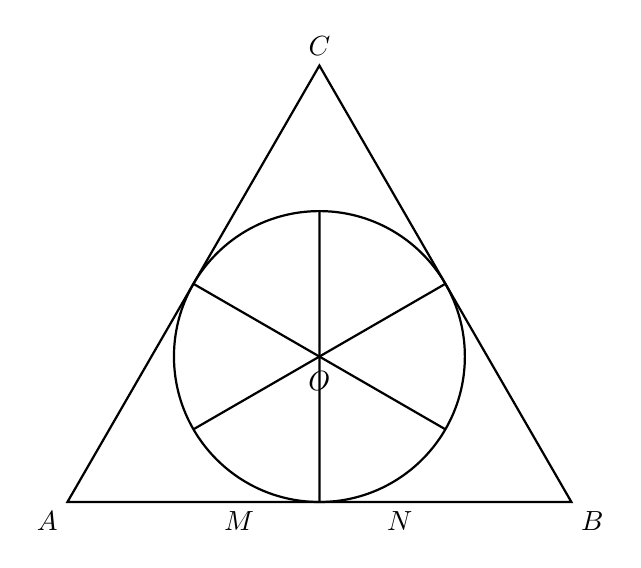
\begin{tikzpicture}[scale=0.8]
  \coordinate (A) at (0,0);
  \coordinate (B) at (8,0);
  \coordinate (C) at (4,6.928);
  \coordinate (O) at (4,2.309);
  \coordinate (M) at (2.9,0);
  \coordinate (N) at (5.1,0);
  \draw[thick] (A) -- (B) -- (C) -- cycle;
  \draw[thick] (O) circle (2.309);
  % bottom spoke (vertical)
  \draw[thick] (O) -- (4,0);
  \draw[thick] (O) -- (4,4.618);
  % spoke 1
  \draw[thick] (O) -- (2.0,1.154);
  \draw[thick] (O) -- (6.0,3.464);
  % spoke 2
  \draw[thick] (O) -- (2.0,3.464);
  \draw[thick] (O) -- (6.0,1.154);
  \node[below left] at (A) {$A$};
  \node[below right] at (B) {$B$};
  \node[above] at (C) {$C$};
  \node[below, yshift=-2pt] at (O) {$O$};
  \node[below, xshift=-4pt] at (M) {$M$};
  \node[below, xshift=4pt] at (N) {$N$};
\end{tikzpicture}
\end{document}
